\glspl{bems} have gained significant attention in recent years due to the increasing need for energy efficiency and sustainability in the built environment.
The primary aim of \glspl{bems} is to monitor, control, and optimize the energy consumption of buildings to reduce energy costs, enhance occupant comfort, and minimize environmental impact.
This section examines the evolution, key components, technologies, benefits, data representation and challenges associated with \glspl{bems}.

\subsection*{Evolution of Building Energy Management Systems}
The concept of \gls{bems} dates back to the 1970s, following the energy crises that highlighted the importance of energy conservation.
Early systems were rudimentary, focusing primarily on basic monitoring and control functions.
With advancements in technology, particularly in \gls{ict}, \glspl{bems} evolved to incorporate more sophisticated features such as real-time data analytics, advanced control algorithms, and integration with renewable energy sources (\cite{Wang2012}).

\subsection*{Key Components and Technologies}
A typical \gls{bems} consists of various components, including sensors, controllers, user interfaces, and communication networks.
Sensors play a critical role in gathering data on parameters such as temperature, humidity, occupancy, and energy usage.
This data is then transmitted to controllers, which process the information and execute control strategies to optimize energy use (\cite{Candanedo2016}).

The integration of \gls{ict} has significantly enhanced the capabilities of \gls{bems}.
Modern systems leverage \gls{iot} devices to enable real-time monitoring and control.
\gls{iot} sensors and smart meters provide granular data, facilitating precise energy management.
Additionally, cloud computing and big data analytics allow for the processing of large volumes of data to identify patterns and anomalies, leading to more efficient energy use (\cite{Bae2021}).
Advanced control strategies, such as \gls{mpc} and \gls{ml} algorithms, have been incorporated into \gls{bems} to improve performance.
\gls{mpc} uses predictive models to forecast future energy demands and adjust control actions accordingly, while \gls{ml} algorithms can optimize energy consumption based on historical data and real-time conditions (\cite{Afram2014}).
\\\gls{ci} in \glspl{bems} plays a crucial role in managing dynamic and diverse requirements of modern buildings.
\gls{ci} algorithms are inherently adept at handling large volumes of heterogeneous data, facilitating anomaly detection, predictive modeling, and optimization, which are essential for maintaining optimal control and occupant comfort.
These algorithms enable \gls{bems} to detect and mitigate suboptimal behaviors, adapt to changing environments, and integrate renewable energy sources efficiently.
Moreover, \gls{ci} techniques such as artificial neural networks, fuzzy logic, and evolutionary algorithms enhance the resilience, security, and overall efficiency of \gls{bems}, ensuring buildings operate optimally even in the face of uncertainties and evolving conditions (\cite{manic2016building}).
Fig. \ref{fig:bems-ci-base-architecture} illustrates a potential framework for employing CI algorithms within a BEMS.

\begin{figure}[htbp]
    \centering
 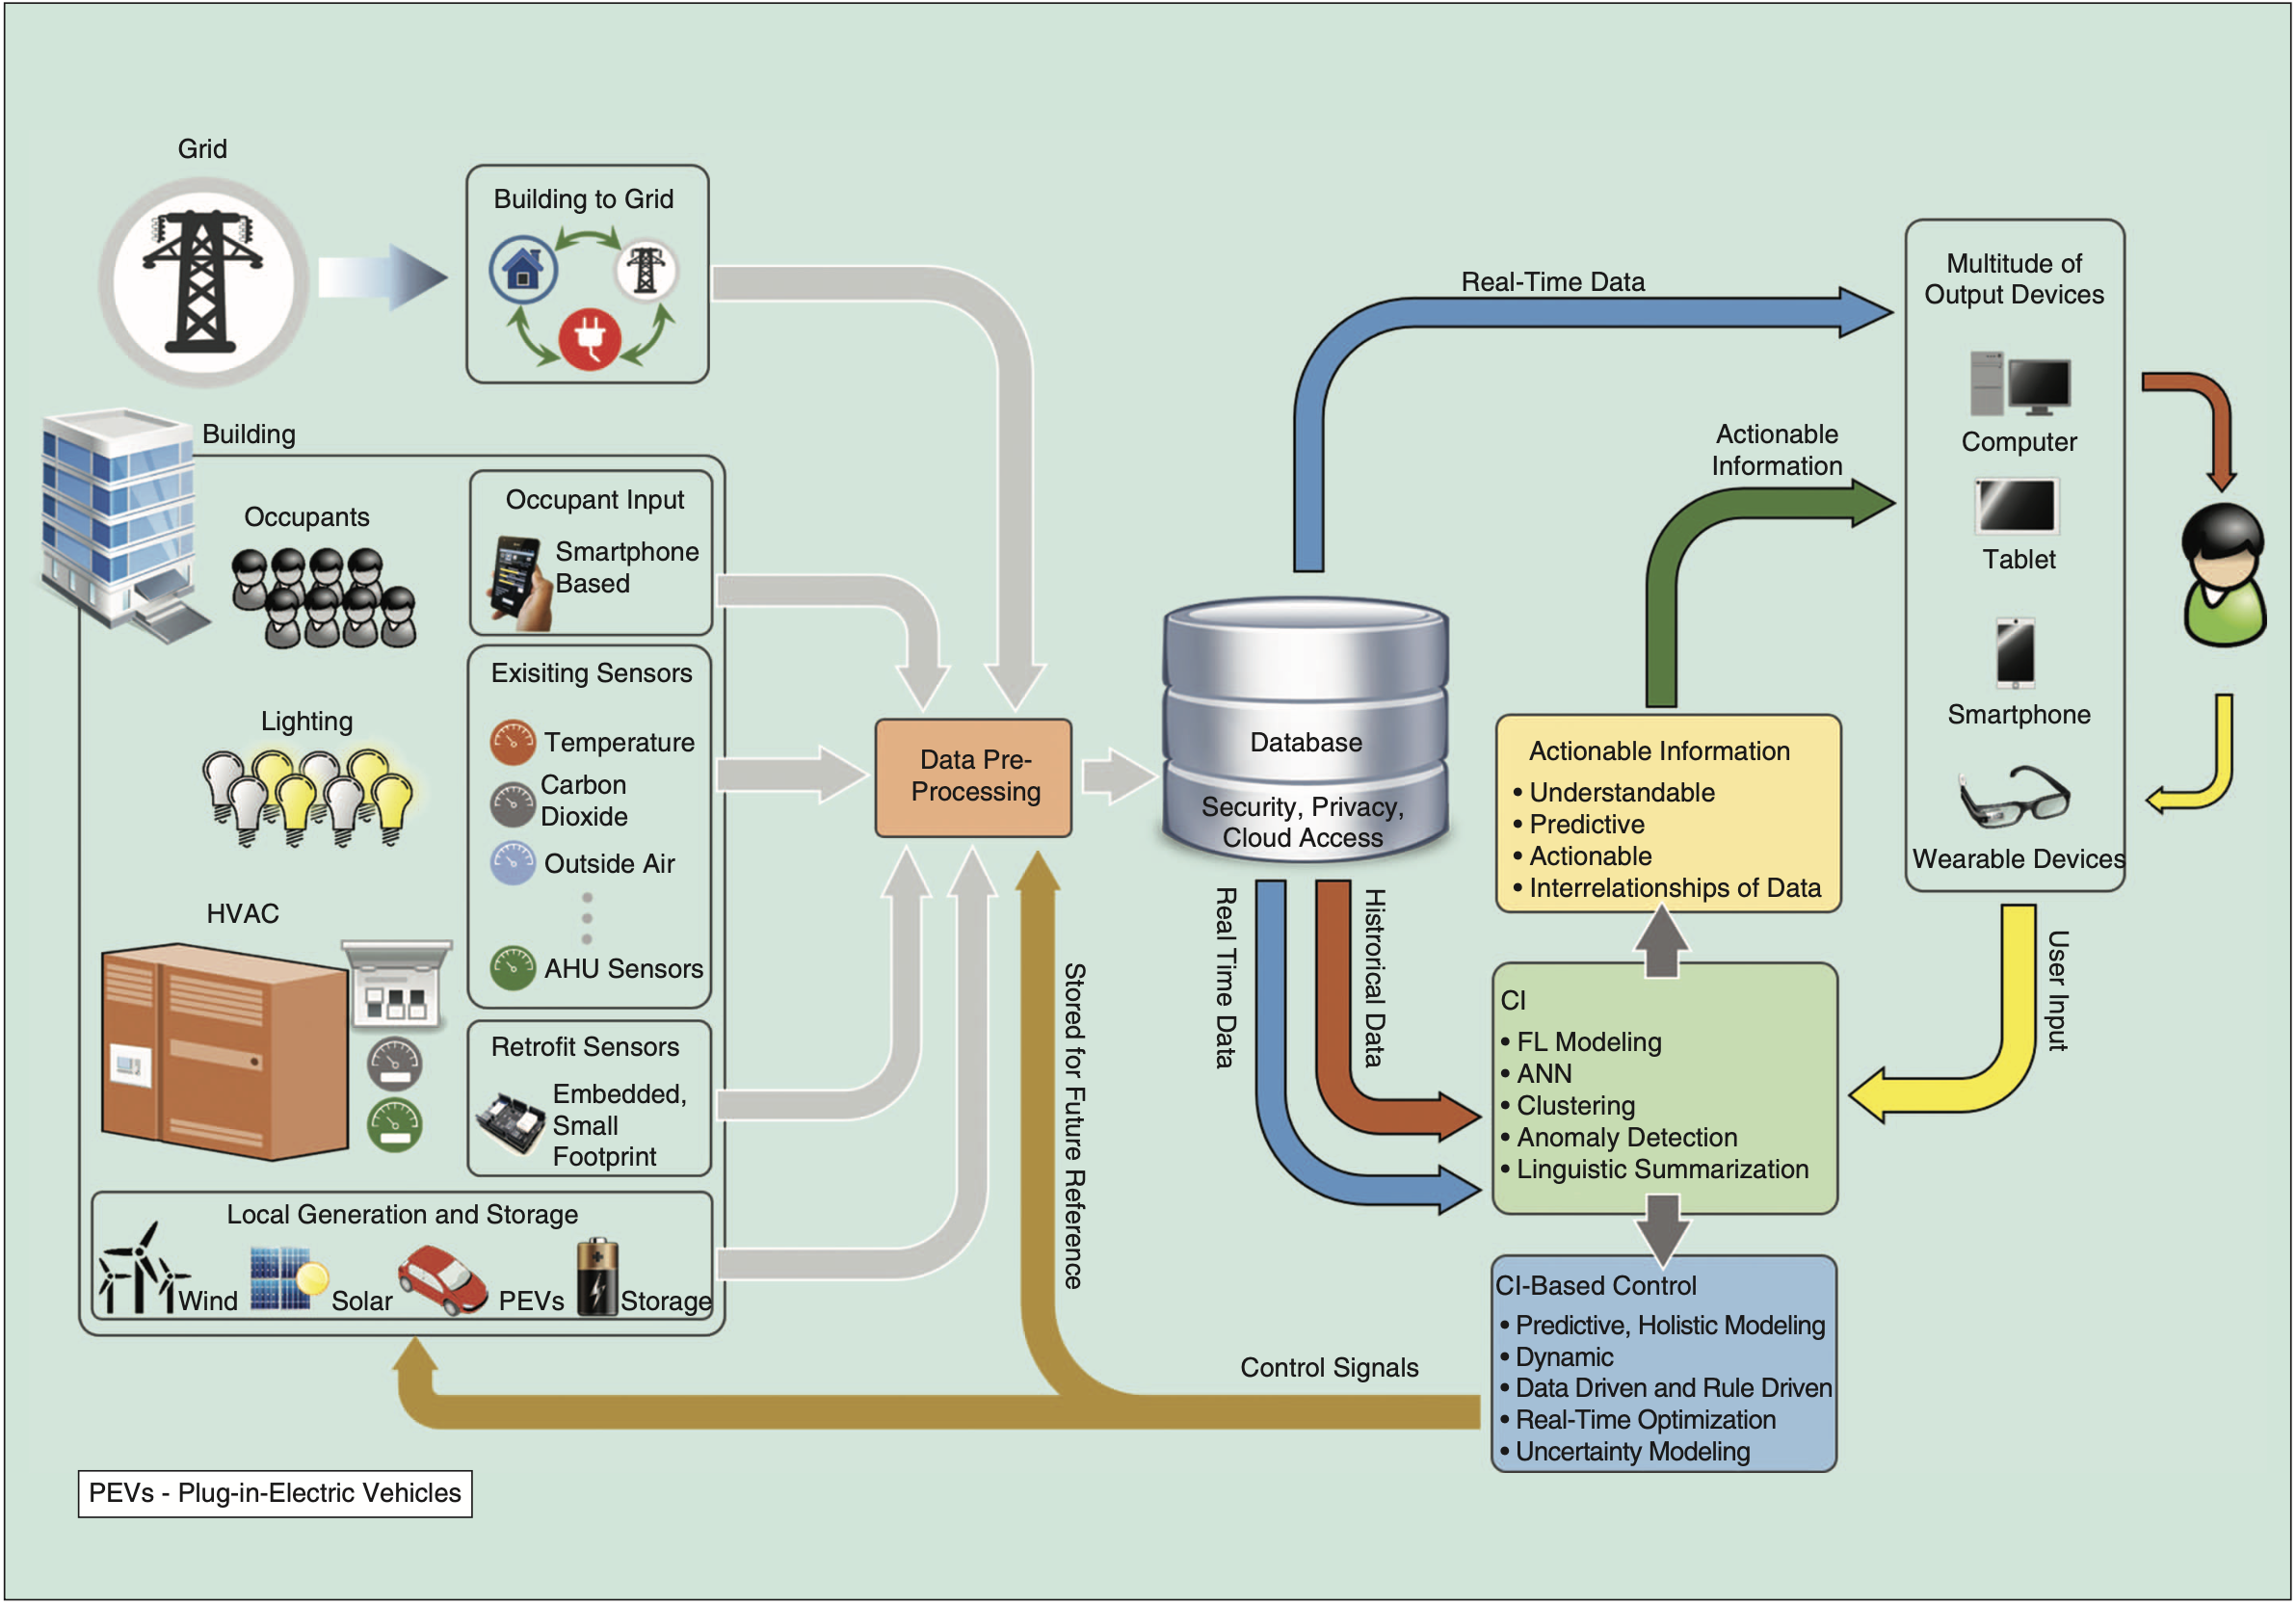
\includegraphics[width=.9\textwidth]{03_Figures/literature-review/bems-ci-based-architecture.png}
     \rule{35em}{0.5pt}
    \caption{A \gls{ci}-based \gls{bems} architecture (\cite{manic2016building})} 
 \label{fig:bems-ci-base-architecture}
\end{figure}

\subsection*{Benefits of Building Energy Management Systems}
The adoption of \gls{bems} offers numerous benefits.
One of the primary advantages is the reduction in energy consumption, which leads to cost savings.
Studies have shown that \gls{bems} can achieve energy savings of up to 30\% in commercial buildings (\cite{Wags2024}).
Moreover, \glspl{bems} enhance occupant comfort by maintaining optimal indoor conditions, such as temperature and air quality.
\gls{bems} also contribute to environmental sustainability by reducing greenhouse gas emissions associated with energy use.
By optimizing energy consumption and integrating renewable energy sources, \gls{bems} can significantly lower a building's carbon footprint (\cite{Lee2016}).
Another benefit is the improved operational efficiency of building systems.
\glspl{bems} enable proactive maintenance by identifying potential issues before they become critical, thereby reducing downtime and maintenance costs (\cite{Klein2012}).

\subsection*{Challenges and Future Directions}
Despite the numerous benefits, the implementation of \gls{bems} faces several challenges.
One of the primary obstacles is the high initial cost of installation and the complexity of integrating \gls{bems} with existing building infrastructure.
Additionally, the effectiveness of \gls{bems} depends on the accuracy and reliability of the data collected by sensors.
Inaccurate or faulty sensors can lead to suboptimal control actions and reduced system performance (\cite{Kokogiannakis2008}).
Cybersecurity is another significant concern, as \glspl{bems} are increasingly connected to the internet and rely on cloud-based services.
According to \cite{Minoli2017}, ensuring the security and privacy of data is critical to prevent unauthorized access and potential cyber-attacks.
Future research and development in \gls{bems} should focus on enhancing interoperability between different systems and devices, developing more robust and scalable control algorithms, and improving the affordability and ease of installation.
The integration of \gls{ai} and \gls{ml} technologies holds promise for further optimizing energy management and improving the adaptability of \gls{bems} to dynamic building conditions (\cite{Amasyali2018}).

\subsection*{Building Data Representation}

According to \cite{Balaji2018}, buildings are responsible for 32\% of global energy consumption.
Recently, a new wave of innovative applications has emerged that utilise a distributed network of sensors, actuators and human interactions to improve building energy efficiency and operations management.
These applications exploit advances in embedded sensing, processing and networking, integrating seamlessly with supervisory control and data acquisition systems in modern buildings and with users on wireless mobile platforms.
However, realising the full potential of smart building applications and cyber-physical systems presents several technical challenges.
One of the main problems is the significant curation required for the sensory data produced by these systems before they can be used effectively.
This curation process is often manual and cost-prohibitive, and hinders widespread adoption due to the absence of a unified descriptive schema.
Recent efforts have attempted to address this problem through data standards and metadata schemas, but often fail to capture the complexity of the relationships required for these applications.
The most relevant ones in the literature and used industrially are discussed below.

\subsubsection*{Brick Ontology}
The Brick ontology is a comprehensive framework designed to standardize the representation of data in buildings, focusing on aspects such as \glspl{bas}, sensors, and equipment (\cite{Balaji2016}).
It addresses the need for a unified data model to facilitate interoperability and integration across various systems within a building.
The ontology provides a schema for representing the physical, logical, and virtual aspects of buildings, which includes the different types of equipment, sensors, and control points, as well as their relationships and properties (\cite{Balaji2018}).
Brick was developed to overcome the challenges posed by the heterogeneity of data formats and schemas used in \glspl{bems}. Traditional \glspl{bems} often suffer from a lack of standardization, leading to difficulties in data integration, system interoperability, and scalable analytics.
Brick ontology addresses these issues by providing a common vocabulary and a structured framework that can be used to describe the different components and their interactions within a building (\cite{Balaji2018}).
The development of Brick ontology has been influenced by several existing models and standards.
It draws inspiration from Project Haystack, a standard for semantic tagging of building data, and the \gls{ifc}, which is a data model used to describe building and construction industry data (\cite{Balaji2016}).
However, Brick extends these models by focusing on a more detailed and formalized representation of building components and their relationships.
The core of Brick ontology consists of three main components: classes, properties, and relationships.
Classes represent the various types of entities found in buildings, such as sensors, HVAC systems, and lighting fixtures.
Properties describe the attributes of these entities, including their states and configurations.
Relationships capture the interactions and connections between different entities, enabling a comprehensive mapping of the building's infrastructure (\cite{Balaji2018}).
Fig. \ref{fig:brick-model-example} illustrates an example of a Brick model, showing the relationships between different building components.
\begin{figure}[htbp]
    \centering
 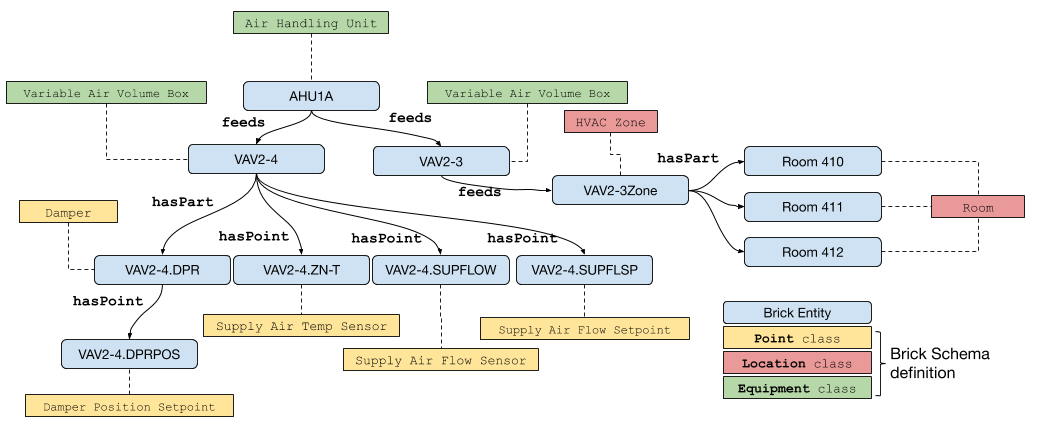
\includegraphics[width=.9\textwidth]{03_Figures/literature-review/brick-model-example.png}
     \rule{35em}{0.5pt}
    \caption{An example of Brick Model (\href{https://docs.brickschema.org/brick/concepts.html}{Brick Ontology Documentation})} 
 \label{fig:brick-model-example}
\end{figure}

The blue nodes represent entities that are instances of Brick classes.
These are the ``things'' within this example of building, encompassing equipment (e.g., AHU1A, VAV2-4), points (e.g., VAV2-4.DPRPOS), locations (e.g., Room 410), and logical collections (e.g., VAV2-3Zone).
The colored boxes, connected to the instances by dashed lines, indicate Brick classes, where the dashed lines represent the ``is an instance of'' relationship (rdf:type).
The solid directed edges depict Brick relationships between entities.

Brick ontology is structured in a way that allows for extensibility and scalability.
New classes and properties can be added to accommodate emerging technologies and new types of equipment.
This flexibility makes Brick a future-proof solution for representing building data, capable of evolving alongside advancements in building automation and smart building technologies (\cite{Balaji2016}).
Several studies and implementations have demonstrated the practical applications of Brick ontology.
For instance, \cite{Balaji2016} illustrated the use of Brick in facilitating the integration of diverse building datasets, enabling advanced analytics and control strategies.
\cite{Balaji2018} further explored the potential of Brick for enhancing energy management systems through improved data interoperability and semantic querying capabilities.
In recent years, Brick has gained significant attention from both academia and industry.
Its adoption is driven by the growing need for more efficient and intelligent building management systems, particularly in the context of smart cities and the \gls{iot} (\cite{Balaji2016}).
By providing a standardized framework, Brick ontology supports the development of innovative solutions for building monitoring, optimization, and automation.
The future prospects of Brick ontology are promising, with ongoing research aimed at enhancing its capabilities and expanding its scope.
Efforts are being made to integrate Brick with other ontologies and data models, such as \gls{saref} and \gls{wot}, to create a more holistic ecosystem for smart building applications (\cite{Balaji2018}).
Additionally, the community-driven development approach of Brick ensures continuous improvement and adaptation to the evolving needs of the building industry.

In conclusion, Brick ontology represents a significant advancement in the field of building data representation.
Its structured and standardized approach addresses the critical challenges of data integration and interoperability in building management systems.
With its extensibility and adaptability, Brick is well-positioned to support the future of smart building technologies and contribute to the development of more efficient and sustainable buildings (\cite{Agarwal2012}; \cite{Balaji2016}; \cite{Balaji2018}).

\subsubsection*{Comparison with Other Building Data Representation Models}
Project Haystack is one of the early initiatives aimed at standardizing the semantic tagging of building data.
It provides a set of tags and conventions for describing the types of equipment, sensors, and operational data found in buildings (\cite{projecthaystack}).
The Haystack tagging model focuses on simplicity and ease of use, allowing practitioners to quickly annotate and share building data.
This approach supports interoperability by ensuring that different systems can understand and process the tagged data consistently.
However, while Project Haystack excels in simplicity, it lacks the formal rigor and extensibility found in more comprehensive ontologies like Brick (\cite{projecthaystack}).

The \gls{ifc} standard, developed by buildingSMART, offers another robust framework for representing building information.
\gls{ifc} is a widely adopted data model that supports the sharing and interoperability of building and construction data throughout the lifecycle of a building (\cite{Liu2021}).
Unlike Brick, which focuses on operational data, \gls{ifc} encompasses a broad range of building information, including architectural, structural, and \gls{mep} components.
\gls{ifc}'s comprehensive nature makes it an essential tool in \gls{bim}, facilitating collaboration among architects, engineers, and contractors (\cite{Liu2021}).
However, its complexity and broad scope can make it challenging to use specifically for \gls{bems} data representation without additional customization.

The \gls{ssn} ontology, developed by the \gls{w3c}, provides a framework for describing sensors and their observations, actuators, and their operations, as well as the systems they are a part of (\cite{Compton2012}).
SSN focuses on the semantic representation of sensor data, enabling the integration and interpretation of sensor information across various applications.
The ontology includes concepts for describing the capabilities, measurements, and deployments of sensors, making it highly suitable for \gls{bems} where sensor data is critical for monitoring and control (\cite{Compton2012}).
However, SSN by itself does not cover the full range of building components and their relationships, which limits its use as a standalone solution for comprehensive \gls{bems} data representation.

Another approach is the \gls{saref} ontology, which provides a common model for representing smart appliances and their functions (\cite{Daniele2015}).
\gls{saref} was developed by ETSI in collaboration with the European Commission to enable interoperability among smart devices.
While \gls{saref} is not exclusively focused on buildings, its application to smart appliances and \gls{iot} devices makes it relevant for smart building scenarios.
The ontology facilitates the integration of various devices and systems, supporting energy management and automation use cases.
\gls{saref}'s modular structure allows for extensions to cover specific domains, including building management, although it may require integration with other ontologies to provide a complete \gls{bems} solution (\cite{Daniele2015}).

In addition to these ontologies, other data representation frameworks and standards have been explored in the context of \gls{bems}.
For instance, the \gls{sos} and the \gls{oandm} standards by the \gls{ogc} provide protocols and data models for accessing and exchanging sensor observations.
These standards enable the integration of spatial and temporal sensor data, which is crucial for building monitoring and analysis.

The development and adoption of these various models highlight the diverse approaches to representing \gls{bems} data.
Each method offers unique strengths and addresses different aspects of building management, from semantic tagging and sensor data integration to comprehensive building information modeling.
The choice of data representation model often depends on the specific requirements of the building management application, including the need for interoperability, the scope of data integration, and the complexity of the building systems involved (\cite{Compton2012,Daniele2015}).
Table \ref{tab:ontology-comparison} provides a comparison of Brick ontology with other building data representation models, highlighting their key aspects and differences.
Table \ref{tab:ontology-comparison-from-brick-ontology-documentation} provides a more detailed comparison of the modeling support offered by Brick, Project Haystack, \gls{ifc}, and \gls{saref}.

In conclusion, while Brick ontology represents a significant advancement in the standardization of building data, it is part of a large ecosystem of models and standards aimed at addressing the diverse needs of \gls{bems}.
Project Haystack, \gls{ifc}, \gls{ssn}, and \gls{saref} each offer distinct approaches to representing building data, contributing to the ongoing efforts to enhance data integration, interoperability, and utilization in \gls{bems}.
By leveraging these various methods, practitioners can develop more efficient, intelligent, and sustainable solutions for managing building operations and energy usage (\cite{Balaji2016,Balaji2018}).

\begin{table}[h!]
    \centering
    \resizebox{\textwidth}{!}{%
    \begin{tabular}{|>{\bfseries}l|l|l|l|l|}
    \hline
    \textbf{Aspect} & \textbf{Brick} & \textbf{SAREF} & \textbf{Project Haystack} & \textbf{IFC} \\
    \hline
    \textbf{Purpose} & Building data model & IoT device interoperability & Building and facility data tagging & Building and construction industry model \\
    \hline
    \textbf{Focus} & Buildings & IoT & Buildings & Construction \\
    \hline
    \textbf{Scope} & Building systems & Smart appliances & Building operations & Entire building lifecycle \\
    \hline
    \textbf{Data Model} & Ontology-based & Ontology-based & Tagging-based & Schema-based \\
    \hline
    \textbf{Standardization} & Open, under development & ETSI standard & Community-driven & ISO standard \\
    \hline
    \textbf{Interoperability} & High & High & Moderate & High \\
    \hline
    \textbf{Ease of Use} & Moderate & High & High & Moderate \\
    \hline
    \textbf{Adoption} & Growing & Moderate & Widely used in building management & Industry standard \\
    \hline
    \end{tabular}%
    }
    \caption{Comparison of Brick, \gls{saref}, Project Haystack, and \gls{ifc}}
    \label{tab:ontology-comparison}
\end{table}

\begin{table}[h!]
    \centering
    \resizebox{\textwidth}{!}{%
    \begin{tabular}{|l|l|l|l|l|}
    \hline
    \textbf{Modeling Support} & \textbf{Brick} & \textbf{Project Haystack} & \textbf{IFC} & \textbf{SAREF}\\
    \hline
    HVAC Systems & \textbf{yes} & \textbf{yes} & \textbf{yes} & no \\
    \hline
    Lighting Systems & \textbf{yes} & partial & \textbf{yes} & no \\
    \hline
    Electrical Systems & \textbf{yes} & \textbf{yes} & \textbf{yes} & no \\
    \hline
    Spatial Information & \textbf{yes} & no & \textbf{yes} & no \\
    \hline
    Sensor Systems & \textbf{yes} & \textbf{yes} & generic & \textbf{yes} \\
    \hline
    Control Relationships & \textbf{yes} & no & generic & no \\
    \hline
    Operational Relationships & \textbf{yes} & no & generic & no \\
    \hline
    Formal Definitions & \textbf{yes} & no & \textbf{yes} & \textbf{yes} \\
    \hline
    \end{tabular}%
    }
    \caption{Modeling Support offered by Brick, Project Haystack, \gls{ifc}, \gls{saref} (\href{https://docs.brickschema.org/intro.html}{Brick Ontology Documentation})}
    \label{tab:ontology-comparison-from-brick-ontology-documentation}
\end{table}

\subsection*{Conclusion}
\glspl{bems} have evolved significantly over the past few decades, driven by advancements in \gls{ict} and the growing need for energy efficiency and sustainability.
Modern \gls{bems} offer numerous benefits, including reduced energy consumption, cost savings, improved occupant comfort, and enhanced environmental sustainability.
However, challenges such as high initial costs, data accuracy, and cybersecurity must be addressed to fully realize the potential of \gls{bems}.
Continued research and innovation are essential to overcome these challenges and advance the capabilities of \gls{bems}, ensuring a sustainable future for the built environment.